\begin{frame}{Le problème Max-Cut 1/2}
Knowing a graph $G=(V ; E)$, made of vertices connected by edges, we want to do the \textit{Maxium Cut}: separate the 
set of vertices $V$ in two complementary parts $V_1$ and $V_2$, so that the set of edges connecting vertices from
$V_1$ and $V_2$ is the largest one. 
\newline

MaxCut can be enhanced by adding \textit{weights} on each edge. It then possible to define a global weight associated with 
a cut. MaxCut will then try to find the cut with the highest global weight.
\centering
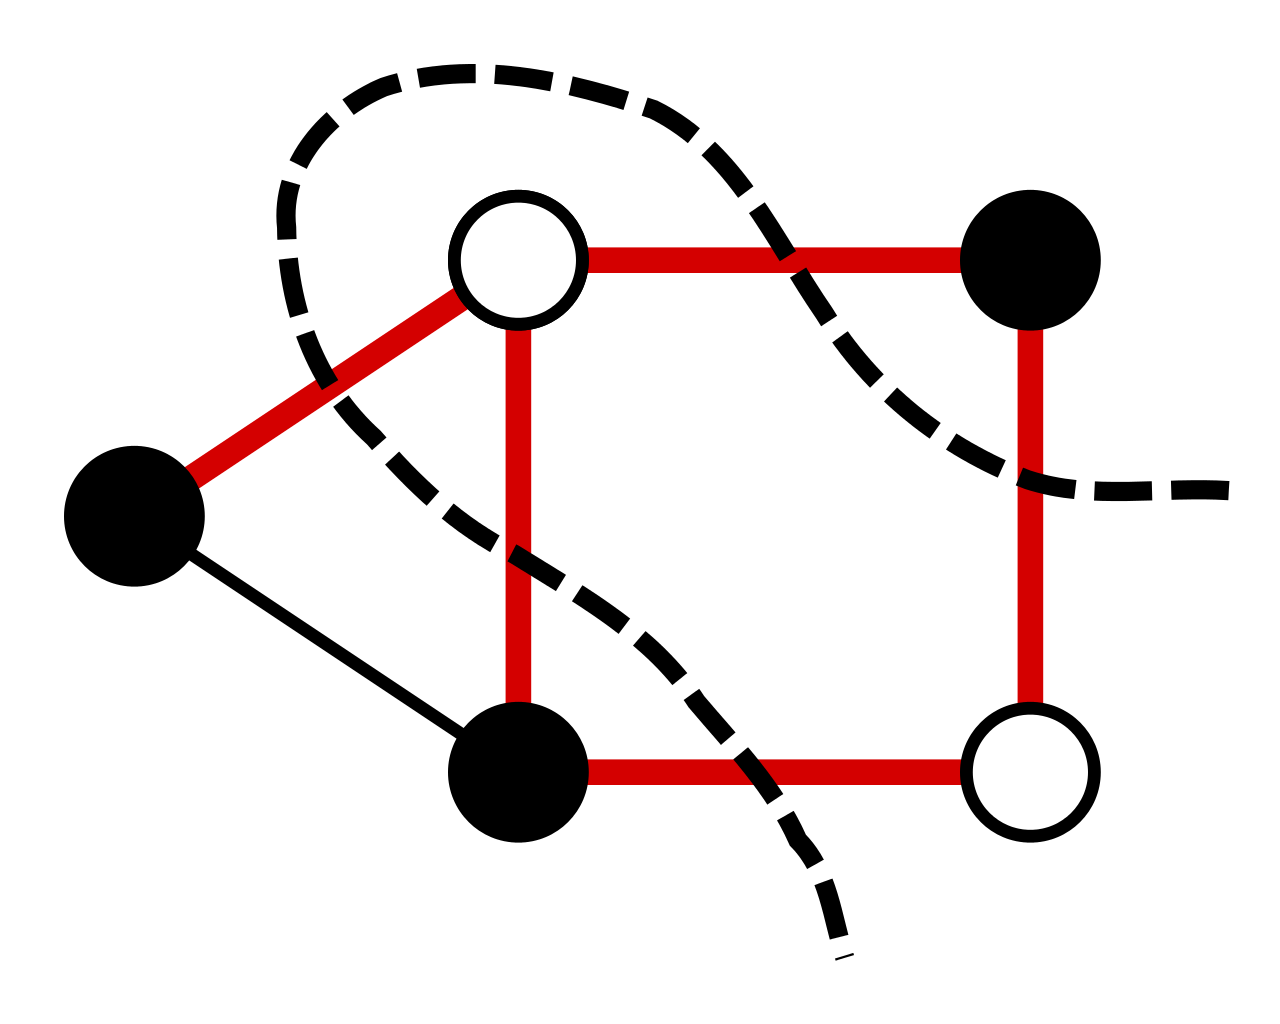
\includegraphics[width=7cm]{images/Max-cut.svg.png}
\end{frame}

\begin{frame}{Le problème Max-Cut 2/2}
\textbf{Remark:} We can define Mincut in a completely similar way.

MaxCut, and the discovery of a maximum cut in a graph is associated with:
\begin{itemize}
    \item decision making problem~: knowing a grap $G$, is there is an integer $k$ such as a cut whose weight is at least $k$
    \item optimisation problem : knowing a graph $G$, find the cut with the highest cut
\end{itemize}

MaxCut has complexity P if the involved graph is \textit{planar} (its dimension is 2); \newline


As graph become more complex, MaxCut is NP-Complete (both NP and NP-hard)
\end{frame}

\begin{frame}{The MIS problem}
Knowing a graphe $G = (V ; E)$, what is the largest set of \textit{independent} vertices, such no edge exist between
any two different elements of this \textit{Maximum Independent Set}.

Sometimes, several different solutions exist 
Il existe souvent plusieurs solutions à ce problème.
\newline

MIS are dominants subsets. A subset of vertices $S$ of a graph is dominant is any vertex is either in $S$, or connected 
(neighbour) to a element in $S$. MIS arte the largets dominant subsets.

\centering
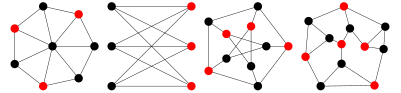
\includegraphics[scale=0.8]{images/MaximumIndependentSet_1000.png}
\end{frame}

\begin{frame}{The MVC problem}
MVC stands for \textit{Maximum Vertex Cover}, it is dual with the MIS problem. 

A cover of vertices is a subset of vertices, it is defined as \textit{transversal} in $G$ if any edge in $E$ connects
to at least one element in the cover. MVC aims to find the smallest transveral cover. 
\newline

Analogy: edges are corridors, verices are "crossroads", where should I installed cameras in order to watch all the 
corridors?

\centering
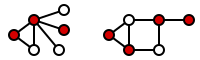
\includegraphics[scale=1.0]{images/Vertex-cover.svg.png}
\end{frame}

\begin{frame}{The SAT problem}
SAT is involved in Cook's theorem's demonstration. Knowing boolean (true or false) variable, we can design a 
\textit{proposition}: a formula using this variables with logicial AND ($\land$) and OR ($\lor$) operator. 
\newline
SAT problem asks this : knowing a proposition, does it have solution? It's not aabout finding solution or counting solutions,
it about knowing if a solution exists. This is why it's call \textit{boolean satisfiability}.
\newline
Example:  $(p\land q)\lor \lnot p$ has result $true$ if $p$ is $false$, with any value for $q$, it can be \textbf{satisfied},
but $(p\land \lnot p)$ has no solution, it can't be satisfied. 

SAT is P with simple proposition, when the proposition's \textit{atoms} involve only two variables, it's 2-SAT. 2-SAT is P.

3-SAT is NP-Complete. Any larger SAT problem can be converted into 3-SAT by increasing the number of variables. 

\end{frame}

\begin{frame}{NP conversion: solving MacCut with QUBO 1/2}

Let's consider this graph with 4 fours and weighted edges.

\centering
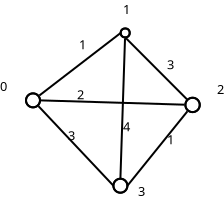
\includegraphics[scale=0.7]{images/graph4pt.png}
\end{frame}

\begin{frame}{NP conversion: solving MacCut with QUBO 2/2}
We can translate the graph into its \textit{connectivity matrix} whose coefficients  $w_{ij}$ are defined by
\begin{itemize}
    \item 0 if $i = j$ 
    \item the weight of the edge connecting  if $i \neq j$ and an efge exist
    \item 0 if no edge exist between nodes $i$ and $j$
\end{itemize}
In our exqmple, we'll build this matrix
\begin{equation*}
 W = \begin{pmatrix}
         0 & 1 & 2 & 3 \\
         1 & 0 & 3 & 4 \\
         2 & 3 & 0 & 1 \\
         3 & 4 & 1 & 0 \\
     \end{pmatrix}    
\end{equation*}
Knowing a graph cut, input binary $b$ has coefficients $b_i$: $1$ if node $i$ is in the cut, 0 otherwise.
Solving MaxCut can be reduced as solving QUBO using the quadratic function associated with the connectivity matrix.
We'll look for the maximum. 
\end{frame}

\begin{frame}{NP conversion: solving 3-SAT with MIS 1/3}
3-SAT can be solved via a MIS problem. 

Let's consider a conjonctive and normal propositiion involving $n$ variables and $m$ clauses.  

\begin{itemize}
    \item for each clause, a small 3 vertices graph is built, each vertex is a variable or the negate of a variable
    \item those small graph are linked by connected a variable in a 3 vertices graph with its negate in another
    3 vertices graph
\end{itemize}
Example: let's consider  $\lnot x_1 \lor x_2 \lor x_3$, it will be depicted by this graph


\centering
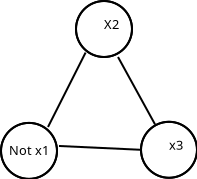
\includegraphics[scale=0.25]{images/Clause3SAT.png}
\end{frame}

\begin{frame}{NP conversion: solving 3-SAT with MIS 2/3}
We connect sub-graphes together by connected $v$ with $\lnot v$

Let's consider
suivante
\begin{equation*}
    (x_1 \lor x_2 \lor x_3) 
    \land (\lnot x_1 \lor x_2 \lor x_3 ) 
    \land (x_1 \lor \lnot x_2 \lor x_3 )
    \land (\lnot x_1 \lor x_2 \lor \lnot x_3 )
\end{equation*}
\centering
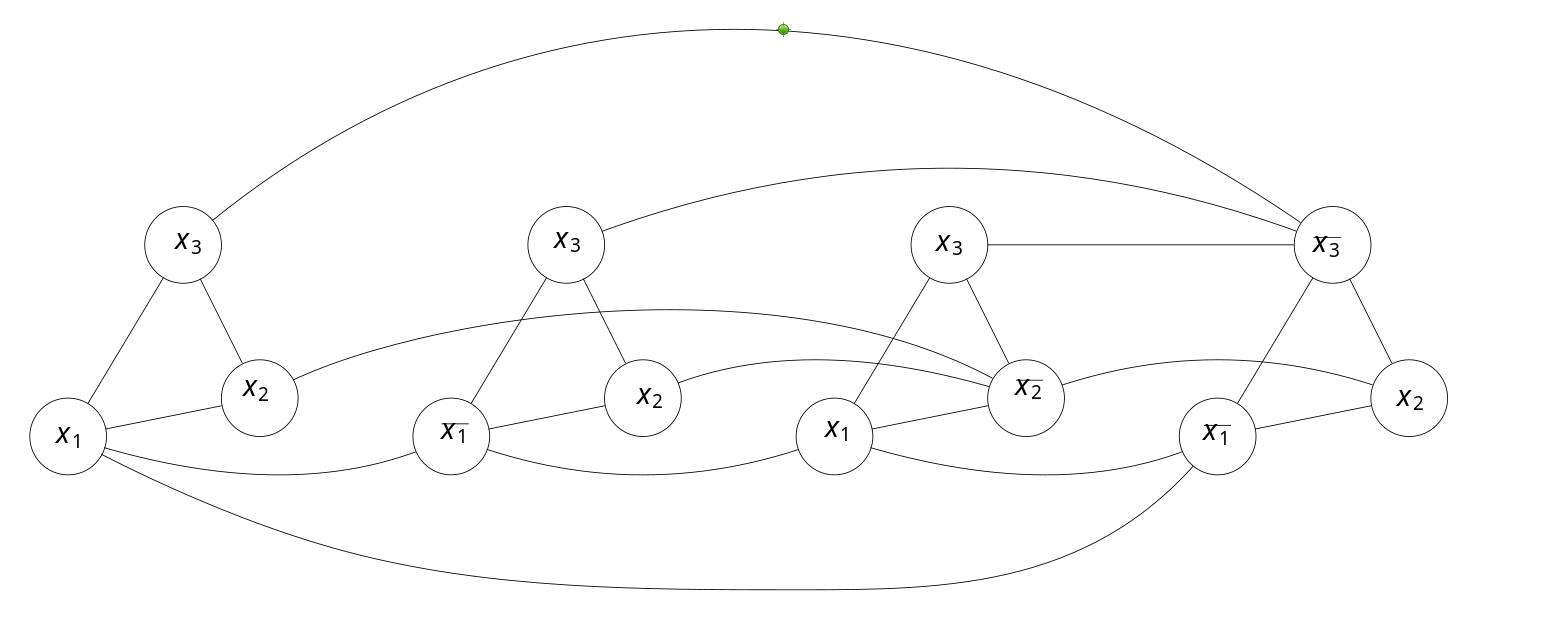
\includegraphics[scale=0.25]{images/Graphe-Clause3SAT.png}
\end{frame}

\begin{frame}{NP conversion: solving 3-SAT with MIS 3/3}
By solving MIS on the resulting graph, we can evaluate the size of this maximum set and compare it to the number of clauses
within the original proposition. If values are the same then the proposition can be satisfied. 


If the MIS size is smallest than the number of clauses, then the proposition can't be satisfied.
\end{frame}

\begin{frame}{NP problems are everywhere}
NP problem are very common in graph theory or in optimisation related problems.

They are often "simple to describe" but "hard to solve".
\begin{itemize}
    \item Traveling Sales Person (TSP) is very interesting for logistics 
    \item Clique problem is very interesting for Social Networks: cliques describe users's community
    \item Many optimisations problem, involving \textit{cost functions}, can be solved as a QUBO
    \item MaxCut is associated with decision making algorithms
\end{itemize}

If any "NP to NPC" conversion is P (Cook's theorem), designing this conversion is very difficult. Many conversion to 
QUBO exist, because QUBO could be approximated since 1984 and was an early point of interest. 
\end{frame}
